\newcommand\auteur{Tony Clavien, Maxime Guillod, Gabriel Luthier \& Guillaume Milani}
\newcommand\cours{GEN}
\newcommand\ecole{IL --- TIC --- HEIG-VD}
\newcommand\domaine{Mini-Projet}
\newcommand\titre{Frogger}
\newcommand\objectif{\item[\textit{Objectif :}]}
\newcommand\duree{\item[\textit{Dur\'ee :}]}
\newcommand\dateRendu{\item[\textit{Date du rendu :}]}
\newcommand\partageTache{\item[\textit{Partage des t\^aches :}]}
\newcommand\effort{\item[\textit{Effort :}]}

\documentclass[a4paper,11pt]{article}
%
\author{\auteur}
\title{\titre}
\date{\today}

\usepackage{fancyhdr}
\usepackage{graphicx}
\usepackage{amsmath}
\usepackage{listings}
\usepackage{listingsutf8}
\usepackage{color}
\usepackage{enumerate}
\usepackage[utf8]{inputenc}
\usepackage[T1]{fontenc}
\usepackage[frenchb]{babel}
\usepackage{float}
\usepackage{geometry}
\usepackage{amssymb,mathtools,pifont}
\usepackage{enumitem}
\usepackage{xspace}
% Liens
\usepackage[hyphens]{url}
\usepackage{hyperref}
\geometry{verbose,tmargin=2.5cm,bmargin=2cm,lmargin=1.8cm,rmargin=1.8cm}
\selectlanguage{frenchb}
\frenchbsetup{StandardLists=true}
\DeclareGraphicsExtensions{.pdf,.png,.jpg}
\setlength\parindent{0pt}
\setlength{\parskip}{0.7em}

\usepackage{color}
\definecolor{light-gray}{gray}{0.95}
\usepackage{listings}
\lstset{
	breaklines=true,
	breakatwhitespace=true,
	backgroundcolor=\color{light-gray}
}

\usepackage{tabularx} % for 'tabularx' environment

% headers & footers
\pagestyle{fancy}

\lhead{\domaine}
\rhead{\titre\space\includegraphics[scale=0.03]{../Logo/Logo.jpg}}

\renewcommand{\footrulewidth}{0.4pt}% default is 0pt
\lfoot{\auteur}
\cfoot{}
\rfoot{\thepage}

%%%%%%%%%%%%%%%%%%%%%%%%%%%%%%%%%%%%%%%
%%%%%%% BEGIN DOCUMENT
%%%%%%%%%%%%%%%%%%%%%%%%%%%%%%%%%%%%%%%

\begin{document}
\clearpage\maketitle
\thispagestyle{empty}

	\maketitle
	\begin{figure}[h!]
		\centering
		
\includegraphics[scale=0.7]{../Logo/logo.jpg}
	\end{figure}
	\newpage

	% % Entete première page
	% \thispagestyle{empty}
	% %
	% \noindent \cours \hfill \ecole{} \newline
	% \noindent \auteur \hfill \today \newline
	% \hrule
	% \vspace{7mm}
	% \noindent {\large \bf \domaine } \hfill \titre {\large \bf }\\[3mm]
	% \hrule

	\tableofcontents
	\listoffigures
	
	% On a pas de tableau
	% \listoftables

	\newpage

	\section{Fonctionnement général}
	\subsection{Objectifs de base}
	Le but de ce projet est de réaliser une application client-serveur dans le cadre du cours GEN. Nous avons décidé de proposer un jeu de type « Frogger » en version valaisanne. \par

	Le but du jeu sera de faire descendre une piste de ski à un Valaisan (\textit{joueur skieur}). Il devra éviter les obstacles la traversant qui seront envoyé par le \textit{défenseur}.


	\begin{figure}[h!]
		\centering
		\fbox{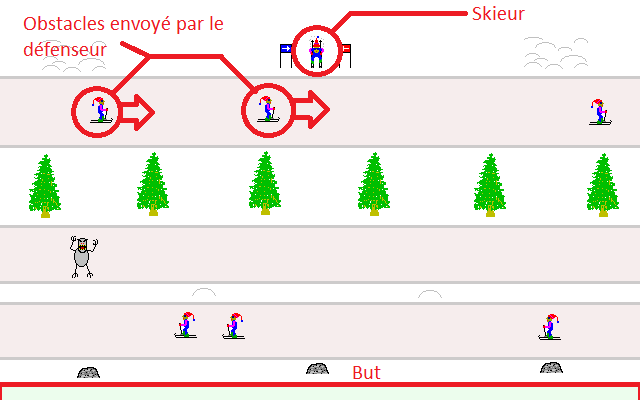
\includegraphics[scale=0.7]{../Screenshots/demo_annotation.png}}
			\caption{Maquette d'une partie}
			\label{maquette}
	\end{figure}

	Les zones rouges sont les zones à disposition du joueur 2 pour placer les obstacles, les sapins sont des obstacles fixes. Le joueur 1 gagne s'il atteint la zone en vert sans heurter d'obstacle.

	\subsection{Utilisation de l'applicatif}
	Le joueur 1 contrôle son personnage à l'aide des flèches du clavier ($\leftarrow \downarrow \rightarrow$) et tente d'éviter les obstacles. Le joueur 2 place les obstacles dans les colonnes, ceci fait que l'obstacle se met en mouvement dans la colonne. Une bouteille de Fendant\texttrademark se vide au fur et à mesure que le joueur 2 place des obstacles. Il doit ensuite attendre qu'elle se remplisse à nouveau pour placer de nouveaux obstacles.\par

	L'administrateur peut régler les paramètres du jeu (« skin » du jeu, vitesse des obstacles, vitesse de rechargement de la bouteille de Fendant\texttrademark). L'administrateur est un rôle hérité de celui de joueur (un administrateur est donc avant tout un joueur). Ce droit est stocké dans la base de données.

	\subsection{Règles du jeu}
	Pour le joueur 1: le but est d'arriver en bas de la piste sans avoir heurté d'obstacle. \\
	Pour le joueur 2: le but est que le joueur 1 heurte un obstacle.

	\subsection{Contraintes}
	Le joueur 1 ne peut pas revenir en arrière, une fois descendu une portion de piste il peut s'arrêter, changer de «colonne» ou de continuer à descendre. \par

	Le joueur 2 peut envoyer des obstacles pour autant que la bouteille de Fendant\texttrademark ne soit pas vide.

	\subsection{Priorités de développement}

	\begin{enumerate}
		\item Première version du jeu «standalone» avec un seul joueur qui prend le rôle du joueur 1 (descendre la piste). Les obstacles sont envoyés aléatoirement. (En parallèle, développement du serveur et de l'API).
		\item Ajout du deuxième joueur en local (les deux jouent sur la même machine avec des touches différentes du clavier).
		\item Les joueurs jouent chacun sur leur machine et se connectent à un serveur distant centralisant la partie. Lorsqu'un joueur se connecte, il voit la liste des parties crées (soit en attente d'un joueur, soit en cours). Il peut soit rejoindre une partie en attente d'un joueur soit créer une nouvelle partie.
		\item L'administrateur peut configurer le serveur (paramètres des parties).
	\end{enumerate}

	\subsection{Base de données}
	La base de données stocke et partage les informations suivantes entre les joueurs et l'administrateur :
	\begin{itemize}
		\item Informations des joueurs (nom d'utilisateur, mot de passe, rôle, points totaux gagnés)
		\item Informations des parties (joueurs, points remportés par chacun)
		\item Paramètres de l'application (ce qui peut être configuré par l'administrateur)
		\item Logs de l'application
	\end{itemize}


	\section{Partage des responsabilité serveur --- client}

	La figure \ref{diagramme_activite} représente le diagramme d'activité qui illustre la répartition des responsabilités entre le client et le serveur.
	\begin{figure}[!ht]
		\centering
		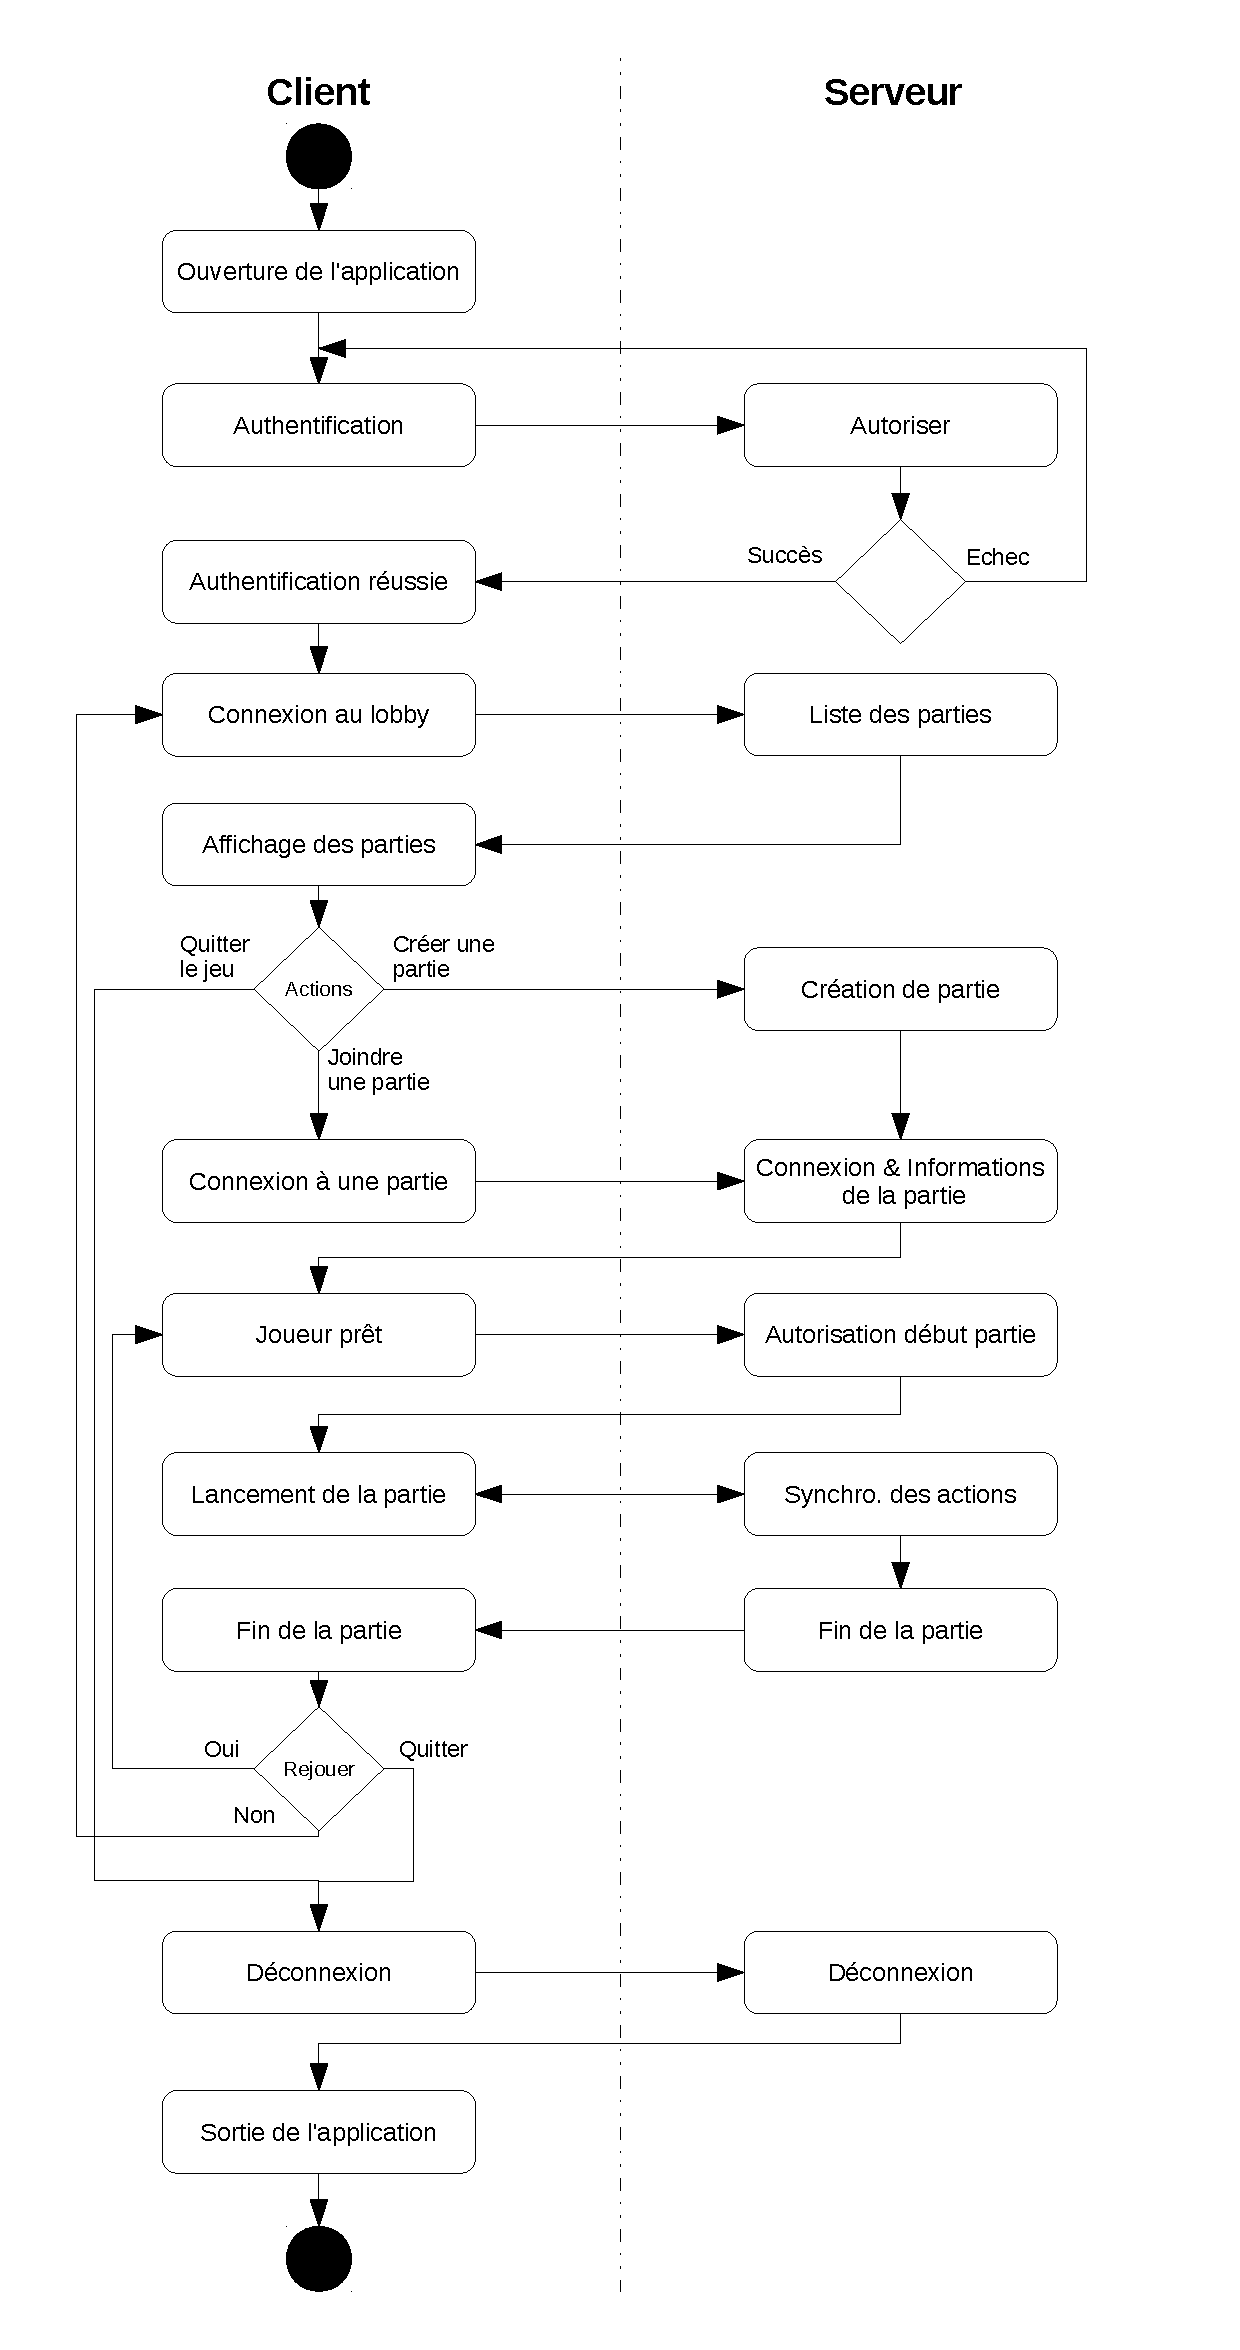
\includegraphics[scale=0.6]{Diagramme_Activite.pdf}
		\caption{Diagramme d'activité}
		\label{diagramme_activite}
	\end{figure}

	\section{Rôle des participants}

		\textbf{Joueurs} : 2 personnes par partie, le \textit{skieur} ayant pour but de réussir à descendre la piste, tandis que l'autre essaye de l'en empêcher (\textit{défenseur}). \\

		\textbf{Administrateur} : Peut changer les règles générales du jeu (configuration des difficulté, tailles des cartes, etc...), et s'occuper des données (nettoyer, modifier des joueurs, etc...)

	\section{Cas d'utilisation}
	
		\begin{figure}[!ht]
			\centering
			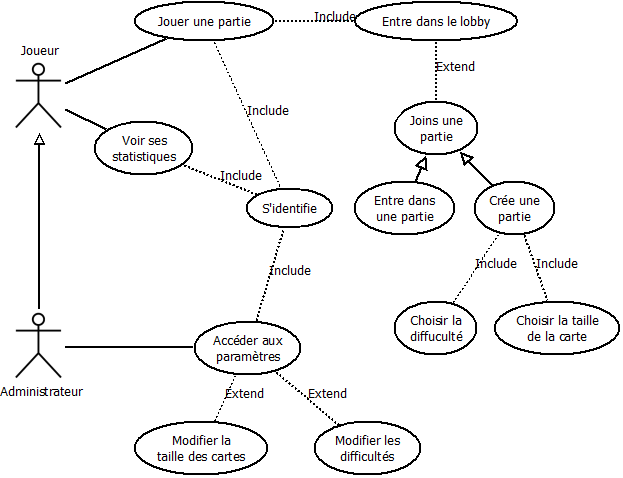
\includegraphics[scale=0.6]{diagramme_utilisation.png}
			\caption{Diagramme d'utilisation}
			\label{diagramme_utilisation}
		\end{figure}
	
		\subsection{Acteurs}
		\begin{enumerate}
			\item Joueurs, dans une partie nommés : \textit{Skieur} et \textit{Défenseur}
			\item Administrateur
		\end{enumerate}
		\subsection{Scénario principal (succès)}
		\begin{enumerate}
			\item L'un des deux joueurs se connecte au lobby et crée une partie en spécifiant les paramètres qu'il souhaite.
			\begin{enumerate}
				\item Difficulté
				\item Taille de la carte
				\item Son rôle (\textit{Skieur} ou \textit{Défenseur})
			\end{enumerate}
			\item Le second joueur rejoint la partie libre du joueur 1 dans le lobby et prends le rôle restant.
			\item Lorsque les 2 joueurs sont prêts la partie commence.
			\begin{enumerate}
				\item "\textit{Le skieur}" tente de traverser la piste en déplaçant son personnage de haut en bas.
				\item "\textit{Le défenseur}" tente de l'en empêcher en envoyant des obstacles de gauche à droite.
				\item La partie se termine si le skieur n'a plus de vie ou si il a atteint l'autre côté (le but).
			\end{enumerate}
			\item À la fin de la partie, soit les rôles s'inversent et on recommence une partie à l'étape 3, soit les joueurs quittent la partie. Cette dernière est donc interrompue et les joueurs retournent au lobby.
		\end{enumerate}

		\subsection{Extensions (ou scénarios alternatifs)}
		Pour permettre la récupération des parties de manière correct, il faut s'assurer que tous les états et les événements sensibles du système peuvent être récupérés à n'importe quelle étape du scénario. \\

		Lors d'une partie, si l'un des deux joueurs est déconnecté, l'adversaire gagne automatiquement la partie et est renvoyé au lobby.

		\subsection{Scénario d'administration}
		\begin{enumerate}
			\item l'administrateur se connecte à l'interface.
			\item Il modifie l'une des options à sa disposition :
			\begin{enumerate}
				\item Les paramètres du jeu.
				\item Les données d'un joueur.
			\end{enumerate}
			\item puis il peut se déconnecte ou recommencer à l'étape 2.
		\end{enumerate}


	\newpage
	\section{Protocole d'échange entre le client et le serveur}
		\subsection{Communication}
			Nous allons utiliser JSON\footnote{JSON : JavaScript Object Notation} comme protocole d'échange entre le client et le serveur. \par
			En effet, de part la structure de son contenu, l'échange d'information entre les deux intervenants est très facilement sérialisable/désérialisable, sans compter sur le fait que le contenu est lisible par un individu (contrairement à un contenu binaire).

		\subsection{Données échangées}
			L'API de communication en cours d'élaboration se trouve sur le wiki de notre projet GitHub \\ \url{https://github.com/gluthier/GEN-projet/wiki/Communication-API} \\
			L'idée est que chaque joueur envoie au serveur ses commandes : pour le skieur s'il souhaite tourner à gauche ou à droite, pour le valaisan sur quelle ligne il envoie un obstacle. Le serveur s'occupe de placer les obstacles et le skieur et envoie les positions de manière régulière aux deux clients. Les clients ne font que l'affichage et l'envoi de commande alors que le serveur s'occupe de la synchronisation, gestion des collisions etc.

	\section{Ébauche du modèle de domaine}
	La figure \ref{model_domain} représente une ébauche du modèle de domaine.

	\begin{figure}[!ht]
		\centering
		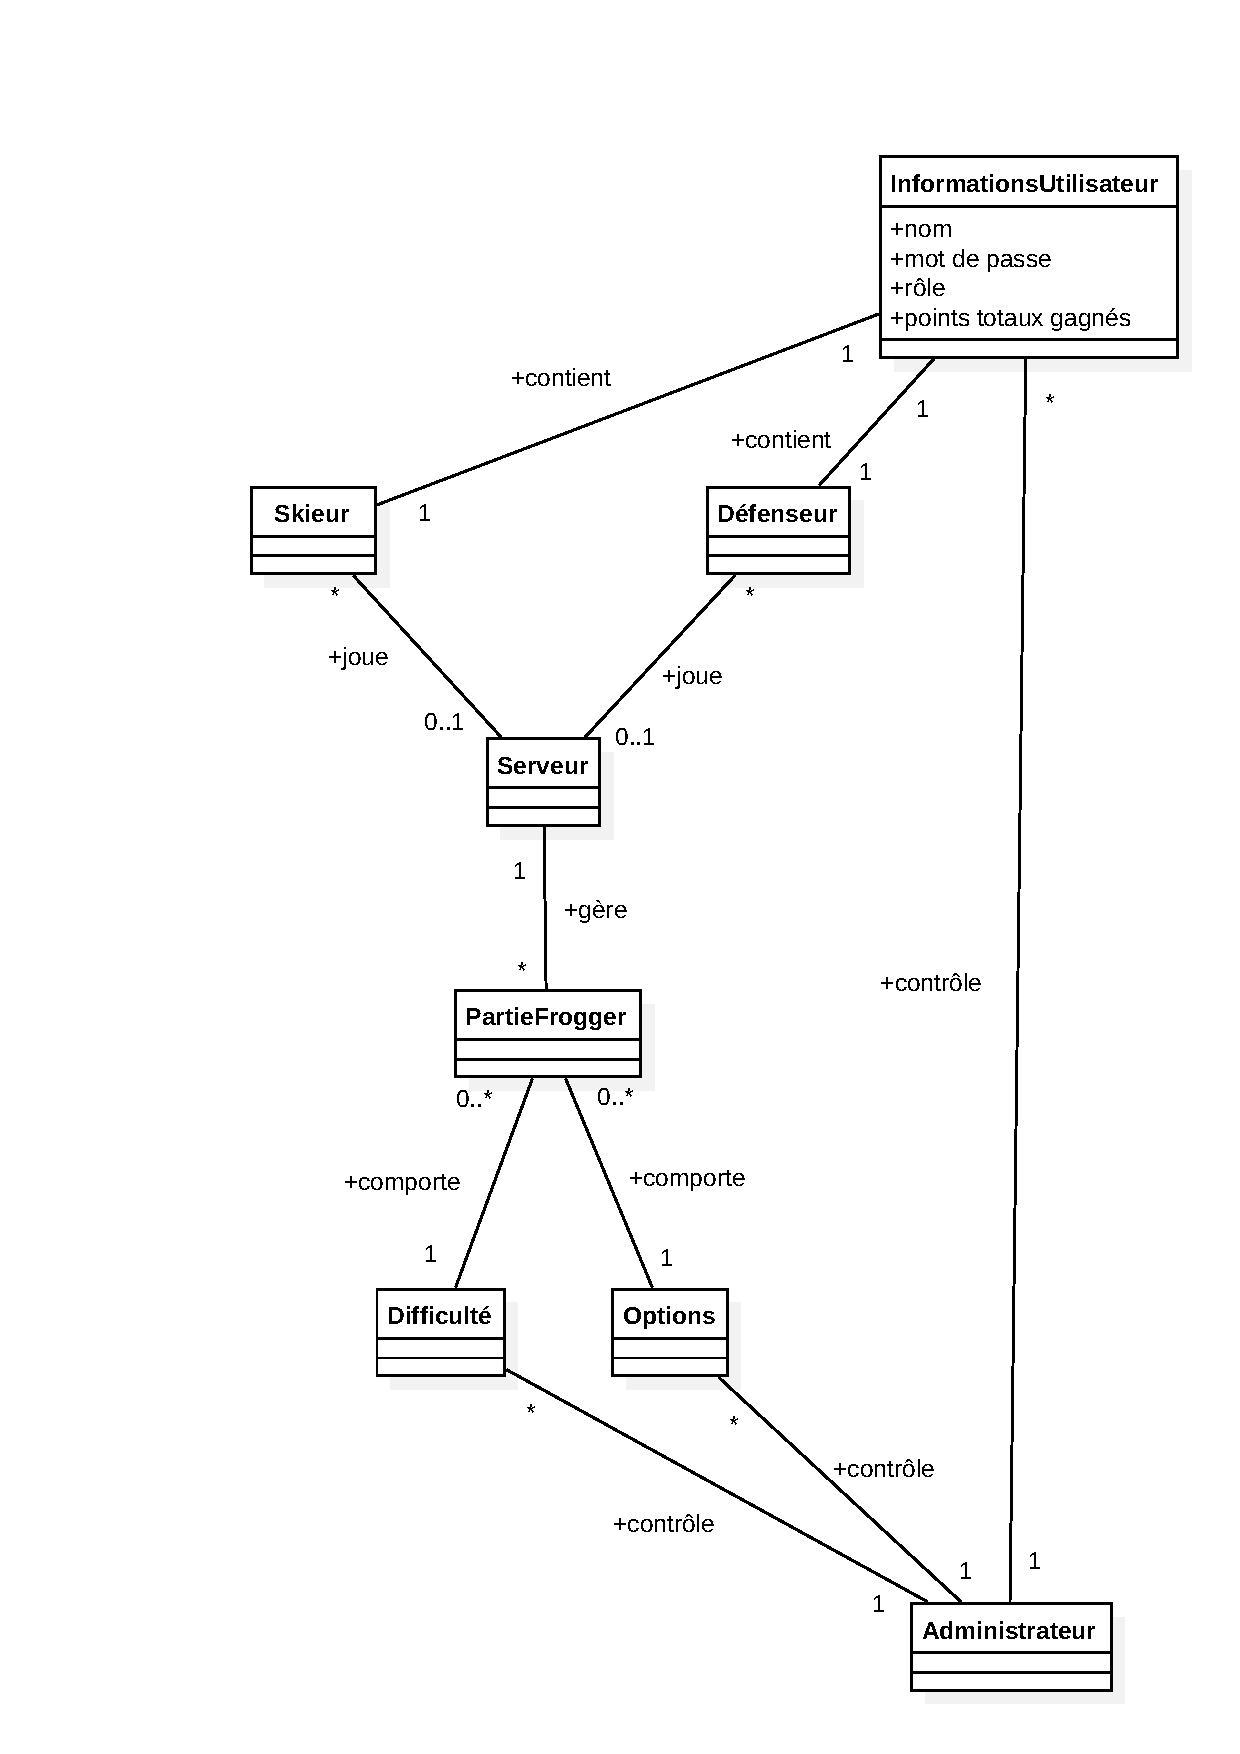
\includegraphics[scale=0.6]{../Schemas/model_domain.pdf}
		\caption{Modèle de domaine}
		\label{model_domain}
	\end{figure}

	\section{Base de donnée}
	L'objectif de la base de données est principalement de stocker les paramètres du jeu et les données utilisateurs. Nous avons fait le choix de ne pas stocker d'informations concernant les parties en cours qui seront chargées uniquement dans la mémoire du serveur. \par

	On trouve donc une entité \texttt{User} qui peut être \texttt{Administrator}, dont on stocke le login et le nombre de victoires. \texttt{Settings} modélise les réglages généraux du jeu, \texttt{MapSize} permettra à l'utilisateur qui créé une partie de choisir parmis plusieurs tailles de carte. \texttt{DifficultyLevel} modélise les niveaux de difficultés parmi lesquels l'utilisateur créant la partie aura le choix.
	\begin{figure}[ht]
		\centering
		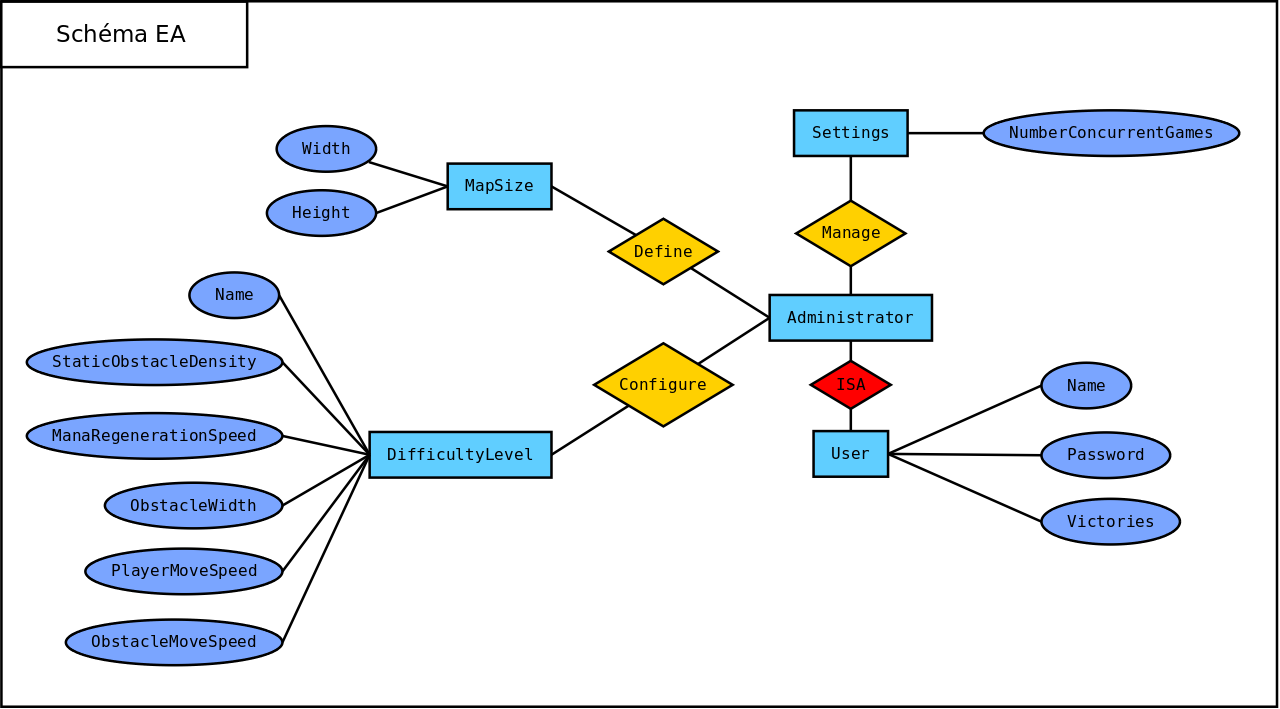
\includegraphics[width=\textwidth]{../Database/ER_diagram.png}
		\caption{Modèle conceptuel}
		\label{database_er}
	\end{figure}

	\section{Rôle des participants}
		\begin{enumerate}
			\item Tony Clavien: Analyste, design manager, programmeur, représentant valaisan
			\item Maxime Guillod: Chef de projet, programmeur
			\item Gabriel Luthier: Responsable des tests, programmeur
			\item Guillaume Milani: Architecte, concepteur en chef, programmeur, community manager
		\end{enumerate}

	\newpage
	\section{Plan d'itération}

		\subsection{Création de l'interface de base}
			\begin{enumerate}[labelwidth=5em,leftmargin=8em]
				\objectif Mise en place de l'interface utilisateur de l'écran principal du jeu.
				\duree 1 semaine
				\dateRendu 26.04.2017
				\partageTache Création des images/sprites, affichage de l'UI, mise en place des obstacles fixes
				\effort 15 heures
			\end{enumerate}
		\subsection{Ajout du 1er joueur avec les obstacles}
		\begin{enumerate}[labelwidth=5em,leftmargin=8em]
			\objectif Développement de la logique du joueur "skieur" qui descend la piste.
			\duree 1 semaine
			\dateRendu 03.05.2017
			\partageTache interaction avec les touches du clavier, déplacement du skieur sur la carte
			\effort 20 heures
		\end{enumerate}
		\subsection{Ajout du 2ème joueur en local}
		\begin{enumerate}[labelwidth=5em,leftmargin=8em]
			\objectif Développement de la logique du joueur "défendant" qui envoie des obstacles contre l'autre joueur.
			\duree 1 semaine
			\dateRendu 10.05.2017
			\partageTache interaction avec les touches du clavier, logique de déplacement des obstacles sur la carte
			\effort 20 heures
		\end{enumerate}
		\subsection{Mise en place des logiques de jeu}
		\begin{enumerate}[labelwidth=5em,leftmargin=8em]
			\objectif Détection des collisions entre les obstacles (fixes et mobiles) avec le joueur "skieur", des conditions de victoire et défaite et barre de recharge pour la pose d'obstacles.
			\duree 1 semaine
			\dateRendu 17.05.2017
			\partageTache détection de collisions, conditions de victoire, conditions de défaite, barre de recharge pour la pose d'obstacles
			\effort 20 heures
		\end{enumerate}
		\subsection{Ajout de la communication avec le serveur}
		\begin{enumerate}[labelwidth=5em,leftmargin=8em]
			\objectif Développement du serveur pour pouvoir jouer à distance.
			\duree 1 semaine
			\dateRendu 24.05.2017
			\partageTache connexion des deux joueurs à une partie, communication réseau entre le serveur et les deux joueurs, gestion de l'état d'une partie
			\effort 30 heures
		\end{enumerate}
		\subsection{Application administrateur}
		\begin{enumerate}[labelwidth=5em,leftmargin=8em]
			\objectif Développement de l'application administrateur utilisée afin de modifier les paramètres des différents modes de jeu et des données des joueurs.
			\duree 1 semaine
			\dateRendu 31.05.2017
			\partageTache UI de l'applicatif, connexion à la base de données, fonctions de modification de la BD
			\effort 20 heures
		\end{enumerate}
		\subsection{Ajout du Lobby}
		\begin{enumerate}[labelwidth=5em,leftmargin=8em]
			\objectif Gestion du lobby (UI et logique).
			\duree 1 semaine
			\dateRendu 07.06.2017
			\partageTache UI du lobby (menu), récupérer les informations sur les parties en recherche de joueurs, création d'une nouvelle partie
			\effort 20 heures
		\end{enumerate}
		\subsection{Finalisation}
		\begin{enumerate}[labelwidth=5em,leftmargin=8em]
			\objectif Finalisation de l'application et ajout de bonus.
			\duree 1 semaine
			\dateRendu 14.07.2017
			\partageTache derniers détails, mise en places des bonus/easter eggs
			\effort 15 heures
		\end{enumerate}

\end{document}
